\section{Thu thập dữ liệu và tiền xử lý dữ liệu}

Dữ liệu phân tích được trích xuất trực tiếp từ \textbf{Binance Public REST API} \cite{binance2024}, endpoint \texttt{/api/v3/klines} cho phép tải về nến ngày của 10 cặp giao dịch (USDT) gồm BTC, ETH, BNB, SOL, XRP, ADA, DOGE, TRX, DOT, MATIC. Mỗi response trả về 13 trường tiêu chuẩn: \texttt{open\_time}, \texttt{open}, \texttt{high}, \texttt{low}, \texttt{close}, \texttt{volume}, \texttt{close\_time}, \texttt{quote\_asset\_volume}, \texttt{number\_of\_trades}, \texttt{taker\_buy\_base\_asset\_volume}, \texttt{taker\_buy\_quote\_asset\_volume} và \texttt{ignore\_field}. Mỗi coin lấy 730 dòng dữ liệu lịch sử (cửa sổ 2 năm gần nhất, tính đến 2026-04-26), riêng MATIC chỉ có dữ liệu đến 09/2024 do bị Binance delist sau khi Polygon rebrand sang POL. Tổng cộng pipeline xử lý $\sim$\textbf{7\,300 dòng dữ liệu thô}.

\subsection{Mục đích}
\hspace*{0.8cm}
Script \texttt{scripts/1\_fetch\_binance.py} là một chương trình Python đảm nhận vai trò \textbf{ingestion layer} -- thu thập dữ liệu giá crypto từ Binance API và chuẩn hoá thành các tệp CSV đồng nhất, sẵn sàng nạp vào tầng Staging của Kho dữ liệu.
Cụ thể, chương trình đảm nhận các chức năng sau:
\begin{itemize}
    \item Gọi Binance REST API có phân trang (limit 1000 nến/request) cho từng cặp coin/USDT.
    \item Chuẩn hoá timestamp Unix mili-giây sang \texttt{datetime} chuẩn ISO.
    \item Ép kiểu dữ liệu cho các cột giá (NUMERIC) và khối lượng (volume base/quote).
    \item Ghi ra các tệp \texttt{raw/<SYMBOL>\_raw.csv} (idempotent, có thể chạy lại nhiều lần).
    \item Ghi log thành công/thất bại để phục vụ debug và audit.
\end{itemize}

\subsection{Các bước xử lý chính}
\begin{enumerate}[label=\alph*)]
    \item \textbf{Cấu hình ban đầu:}
    Đọc cấu hình từ tệp \texttt{.env} (\texttt{PG\_HOST}, \texttt{PG\_PORT}, \texttt{PG\_DATABASE}, \texttt{PG\_USER}, \texttt{PG\_PASSWORD}). Danh sách 10 cặp giao dịch (\texttt{TICKERS}) được khai báo cứng trong script.

    \item \textbf{Các hàm hỗ trợ trong \texttt{scripts/parsers.py}:}
    Chương trình tái sử dụng các hàm parser từ dự án trước:
    \begin{itemize}
        \item \texttt{parse\_number}: Chuẩn hoá chuỗi số có chứa dấu phẩy/chấm (ví dụ ``63{,}770.00'' $\rightarrow$ 63770.0).
        \item \texttt{parse\_date}: Chuẩn hoá chuỗi ngày sang \texttt{datetime}.
        \item \texttt{parse\_volume}: Quy đổi chuỗi ``1.2M'', ``900K'' về số nguyên tuyệt đối.
    \end{itemize}

    \item \textbf{Gọi API và tải dữ liệu:}
    Với mỗi coin, chương trình gửi HTTP GET tới endpoint \texttt{/api/v3/klines} với tham số \texttt{symbol=<SYMBOL>USDT}, \texttt{interval=1d}, \texttt{limit=1000}. Tự động retry tối đa 3 lần khi lỗi mạng hoặc rate-limit (HTTP 429).

    \item \textbf{Xử lý từng coin:}
    Sau khi nhận response JSON, chương trình:
    \begin{itemize}
        \item Convert thời gian từ Unix milliseconds sang \texttt{open\_time}/\texttt{close\_time} kiểu \texttt{datetime}.
        \item Ép kiểu \texttt{NUMERIC(18,8)} cho cột \texttt{open}, \texttt{high}, \texttt{low}, \texttt{close} và \texttt{NUMERIC(20,4)} cho \texttt{volume}, \texttt{quote\_asset\_volume}.
        \item Tính các metric phái sinh ở tầng Transform (qua Pentaho hoặc SQL fallback):
        \begin{itemize}
            \item \textbf{Return\_pct:} $(Close - Open) / Open \times 100$
            \item \textbf{Volume\_USD:} $Close \times Volume$
            \item \textbf{Volatility:} $High - Low$
            \item \textbf{Average\_price:} $(High + Low) / 2$
            \item \textbf{Log\_return:} $\ln(Close) - \ln(Open)$
            \item \textbf{Z\_score\_close:} $(Close - \mu_{30}) / \sigma_{30}$ với cửa sổ rolling 30 ngày
            \item \textbf{Is\_anomaly:} $|z\_score| > 2$
        \end{itemize}
        \item Sắp xếp theo \texttt{open\_time} tăng dần và lưu ra \texttt{raw/<SYMBOL>\_raw.csv}.
    \end{itemize}

    \item \textbf{Tải lên Staging và Gold:}
    Sau khi 10 file CSV được sinh xong, pipeline gọi \texttt{psql \textbackslash copy} (hoặc Pentaho job \texttt{01\_clean.kjb}) để nạp vào \texttt{staging.ohlcv\_raw}. Tiếp theo, script \texttt{02\_transform\_fallback.sql} (hoặc \texttt{02\_transform.kjb}) tính các metric và đẩy vào \texttt{staging.fact\_prep}. Cuối cùng \texttt{03\_load\_gold.sql} thực hiện \texttt{TRUNCATE + INSERT} vào \texttt{gold.fact\_market\_daily}.
\end{enumerate}

\subsection{Kết quả đầu ra}
\begin{itemize}
    \item 10 tệp CSV thô tại \texttt{raw/<SYMBOL>\_raw.csv} -- đầu vào cho Pentaho/SQL.
    \item Bảng \texttt{staging.ohlcv\_raw} chứa $\sim$7\,300 dòng dữ liệu đã chuẩn hoá kiểu.
    \item Bảng \texttt{gold.fact\_market\_daily} (Star Schema) sẵn sàng cho OLAP và Data Mining.
    \item 3 OLAP view: \texttt{v\_weekly\_return\_by\_category}, \texttt{v\_volume\_leaderboard}, \texttt{v\_top\_anomalies}.
\end{itemize}

\begin{figure}[H]
    \centering
    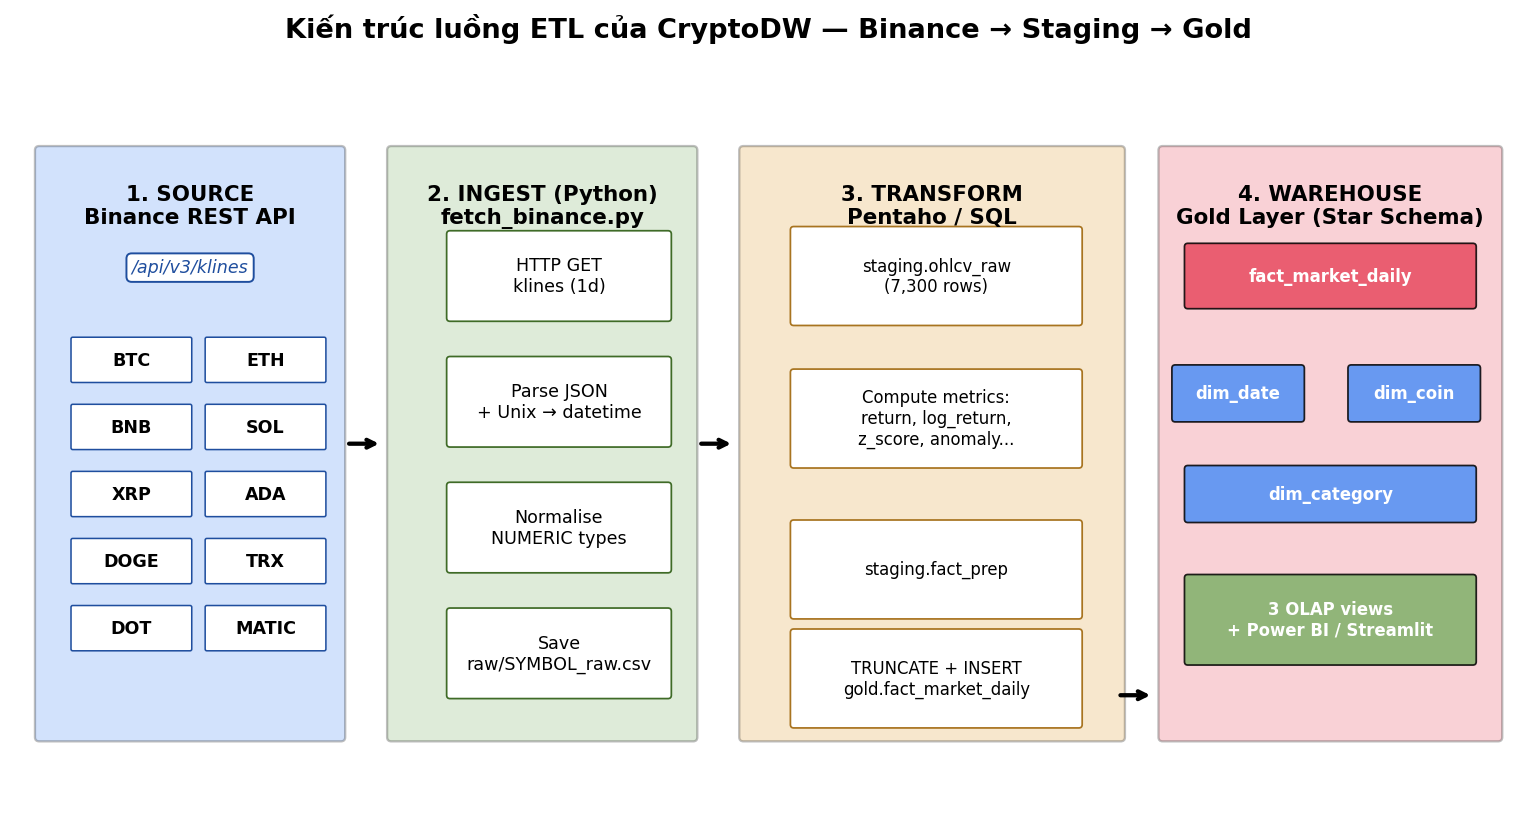
\includegraphics[width=0.9\textwidth]{Images/etl_diagram.png}
    \caption{Kiến trúc luồng dữ liệu ETL và cấu trúc Schema của Kho dữ liệu Crypto}
    \label{fig:etl_architecture}
\end{figure}

\subsection{Thiết kế kho dữ liệu}

\subsubsection{Mô hình dữ liệu (Star Schema)}

\begin{figure}[H]
    \centering
    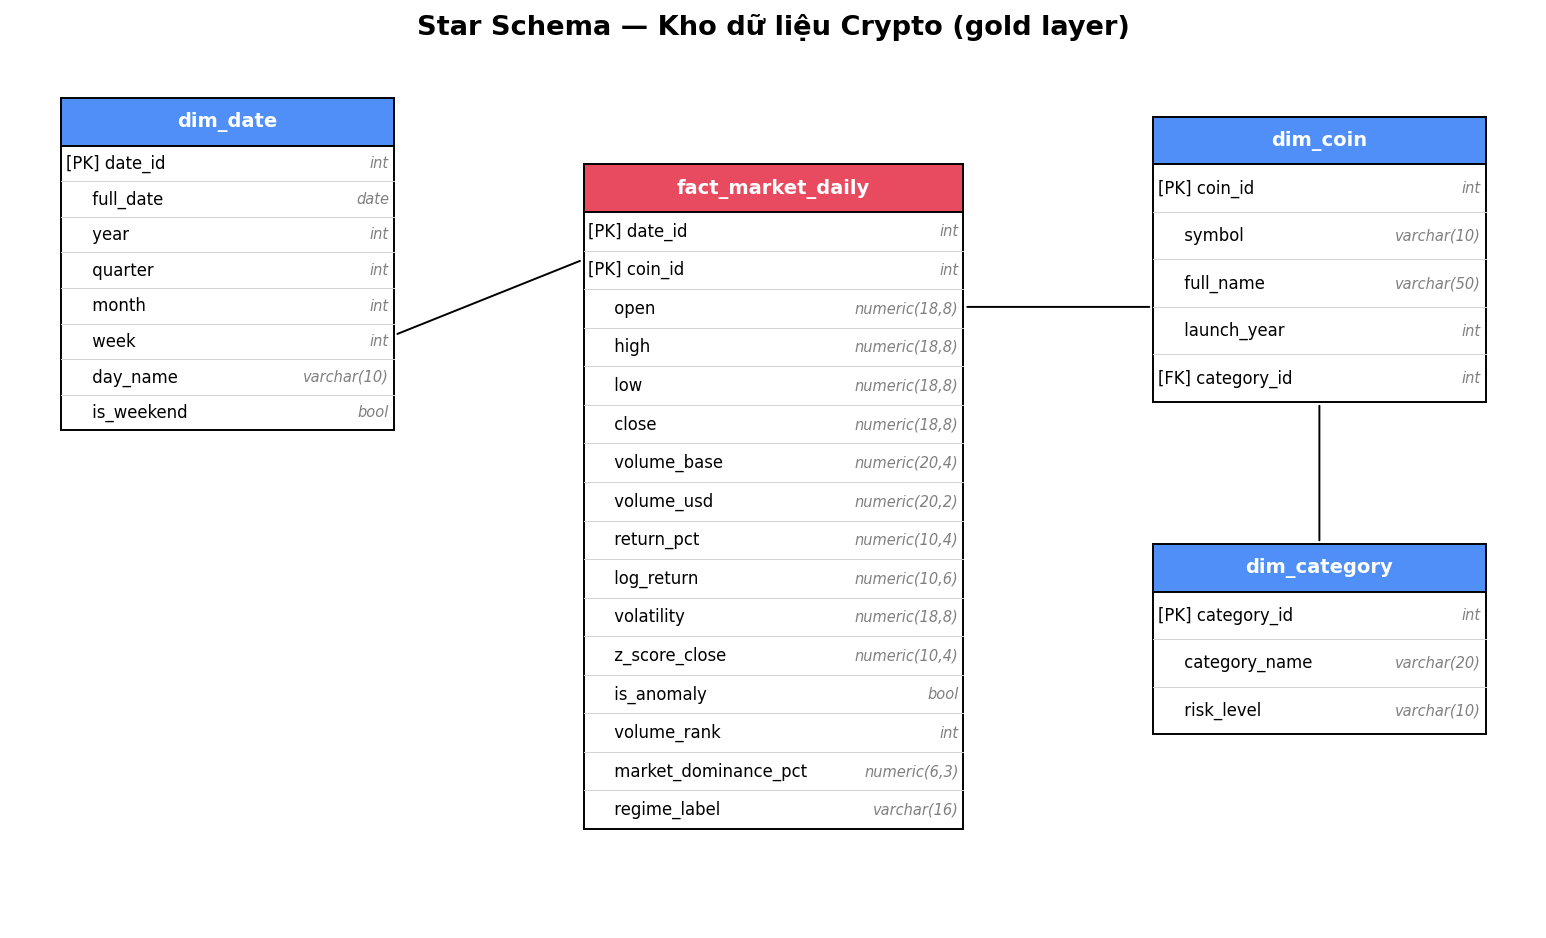
\includegraphics[width=0.9\textwidth]{Images/star-dwh.png}
    \caption{Mô hình kiến trúc Star Schema cho Kho dữ liệu Crypto}
    \label{fig:star_schema_design}
\end{figure}

Dựa trên đặc thù dữ liệu thị trường tiền mã hoá (giao dịch 24/7, biến động cao, phân hoá nhóm rõ rệt) và nhu cầu phân tích đa chiều, nhóm lựa chọn kiến trúc \textbf{Star Schema} -- mô hình được khuyến nghị cho data warehouse phân tích bởi Kimball \cite{kimball2013} và được Inmon coi là ``physical implementation tự nhiên'' cho dimensional modeling \cite{inmon2005}. Mô hình bao gồm một bảng \textit{Fact Table} trung tâm \texttt{fact\_market\_daily} kết nối trực tiếp với ba bảng chiều \textit{Dimension Tables}: \texttt{dim\_date}, \texttt{dim\_coin} và \texttt{dim\_category}.

Các lý do chính cho việc lựa chọn Star Schema thay vì Snowflake Schema bao gồm:
\begin{itemize}
    \item \textbf{Tối ưu hoá hiệu suất truy vấn:} Star Schema giảm thiểu số JOIN. Với mục tiêu so sánh nhanh giữa các nhóm L1, L2, Meme, Payment, việc phi chuẩn hoá thông tin \texttt{category\_name} và \texttt{risk\_level} ngay trong \texttt{dim\_category} (không tách thêm bảng phụ) giúp truy vấn nhanh hơn.
    \item \textbf{Đơn giản hoá cho người dùng cuối:} Cấu trúc đơn giản giúp các công cụ BI (Power BI, Streamlit) dễ dàng mô hình hoá và tương tác.
    \item \textbf{Phù hợp quy mô dữ liệu:} Với 10 coin và 4 category, việc chuẩn hoá quá mức không mang lại lợi ích về lưu trữ.
\end{itemize}

\subsubsection{Chi tiết thiết kế các bảng (Star Schema)}

\begin{table}[H]
\centering
\caption{Đặc tả bảng sự kiện: \texttt{gold.fact\_market\_daily}}
\label{tab:fact_market_daily}
\resizebox{\textwidth}{!}{%
\begin{tabular}{@{}llll@{}}
\toprule
\textbf{Tên trường} & \textbf{Kiểu dữ liệu} & \textbf{Ràng buộc} & \textbf{Mô tả} \\ \midrule
date\_id & int & PK, FK & Khóa ngoại $\rightarrow$ \texttt{dim\_date} \\
coin\_id & int & PK, FK & Khóa ngoại $\rightarrow$ \texttt{dim\_coin} \\
open & numeric(18,8) & & Giá mở phiên \\
high & numeric(18,8) & & Giá cao nhất \\
low & numeric(18,8) & & Giá thấp nhất \\
close & numeric(18,8) & & Giá đóng phiên \\
volume\_base & numeric(20,4) & & Khối lượng đơn vị coin \\
volume\_usd & numeric(20,2) & & $close \times volume\_base$ \\
return\_pct & numeric(10,4) & & $(close-open)/open \times 100$ \\
log\_return & numeric(10,6) & & $\ln(close) - \ln(open)$ \\
volatility & numeric(18,8) & & $high - low$ \\
average\_price & numeric(18,8) & & $(high+low)/2$ \\
z\_score\_close & numeric(10,4) & & Z-Score rolling 30 ngày \\
is\_anomaly & boolean & & $|z\_score| > 2$ \\
volume\_rank & int & & RANK theo \texttt{volume\_usd} mỗi ngày \\
market\_dominance\_pct & numeric(6,3) & & $volume\_usd / SUM(\text{ngày}) \times 100$ \\
regime\_label & varchar(16) & & Bull / Bear / Sideways \\ \bottomrule
\end{tabular}%
}
\end{table}

\begin{table}[H]
\centering
\caption{Đặc tả bảng chiều: \texttt{gold.dim\_coin}}
\label{tab:dim_coin}
\begin{tabular}{@{}llll@{}}
\toprule
\textbf{Tên trường} & \textbf{Kiểu dữ liệu} & \textbf{Ràng buộc} & \textbf{Mô tả} \\ \midrule
coin\_id & int & PK & Khoá đại diện \\
symbol & varchar(10) & NN, UQ & Mã giao dịch (BTC, ETH, ...) \\
full\_name & varchar(50) & & Tên đầy đủ (Bitcoin, Ethereum, ...) \\
launch\_year & int & & Năm ra mắt \\
category\_id & int & FK & $\rightarrow$ \texttt{dim\_category} \\ \bottomrule
\end{tabular}
\end{table}

\begin{table}[H]
\centering
\caption{Đặc tả bảng chiều: \texttt{gold.dim\_category}}
\label{tab:dim_category}
\begin{tabular}{@{}llll@{}}
\toprule
\textbf{Tên trường} & \textbf{Kiểu dữ liệu} & \textbf{Ràng buộc} & \textbf{Mô tả} \\ \midrule
category\_id & int & PK & Khoá nhóm \\
category\_name & varchar(20) & NN & L1 / L2 / Meme / Payment \\
risk\_level & varchar(10) & & Low / Mid / High \\ \bottomrule
\end{tabular}
\end{table}

\begin{table}[H]
\centering
\caption{Đặc tả bảng chiều thời gian: \texttt{gold.dim\_date}}
\label{tab:dim_date}
\begin{tabular}{@{}llll@{}}
\toprule
\textbf{Tên trường} & \textbf{Kiểu dữ liệu} & \textbf{Ràng buộc} & \textbf{Mô tả} \\ \midrule
date\_id & int & PK & Định dạng YYYYMMDD \\
full\_date & date & NN & Ngày đầy đủ \\
year & int & & Năm \\
quarter & int & & Quý (1--4) \\
month & int & & Tháng (1--12) \\
month\_name & varchar(10) & & Jan, Feb, ... \\
day\_of\_month & int & & Ngày trong tháng \\
day\_name & varchar(10) & & Monday, Tuesday, ... \\
is\_weekend & bool & & Cờ cuối tuần \\ \bottomrule
\end{tabular}
\end{table}

\subsubsection{Phương án thay thế: Mô hình Snowflake Schema}

Bên cạnh Star Schema, nhóm cũng xem xét mô hình \textbf{Snowflake Schema} (Lược đồ bông tuyết). Trong phương án này, bảng \texttt{dim\_coin} có thể được tách thêm các sub-dimension như \texttt{dim\_blockchain} (cơ chế đồng thuận: PoW, PoS) hoặc \texttt{dim\_protocol} (Bitcoin, EVM, Solana VM, ...).

\begin{figure}[H]
    \centering
    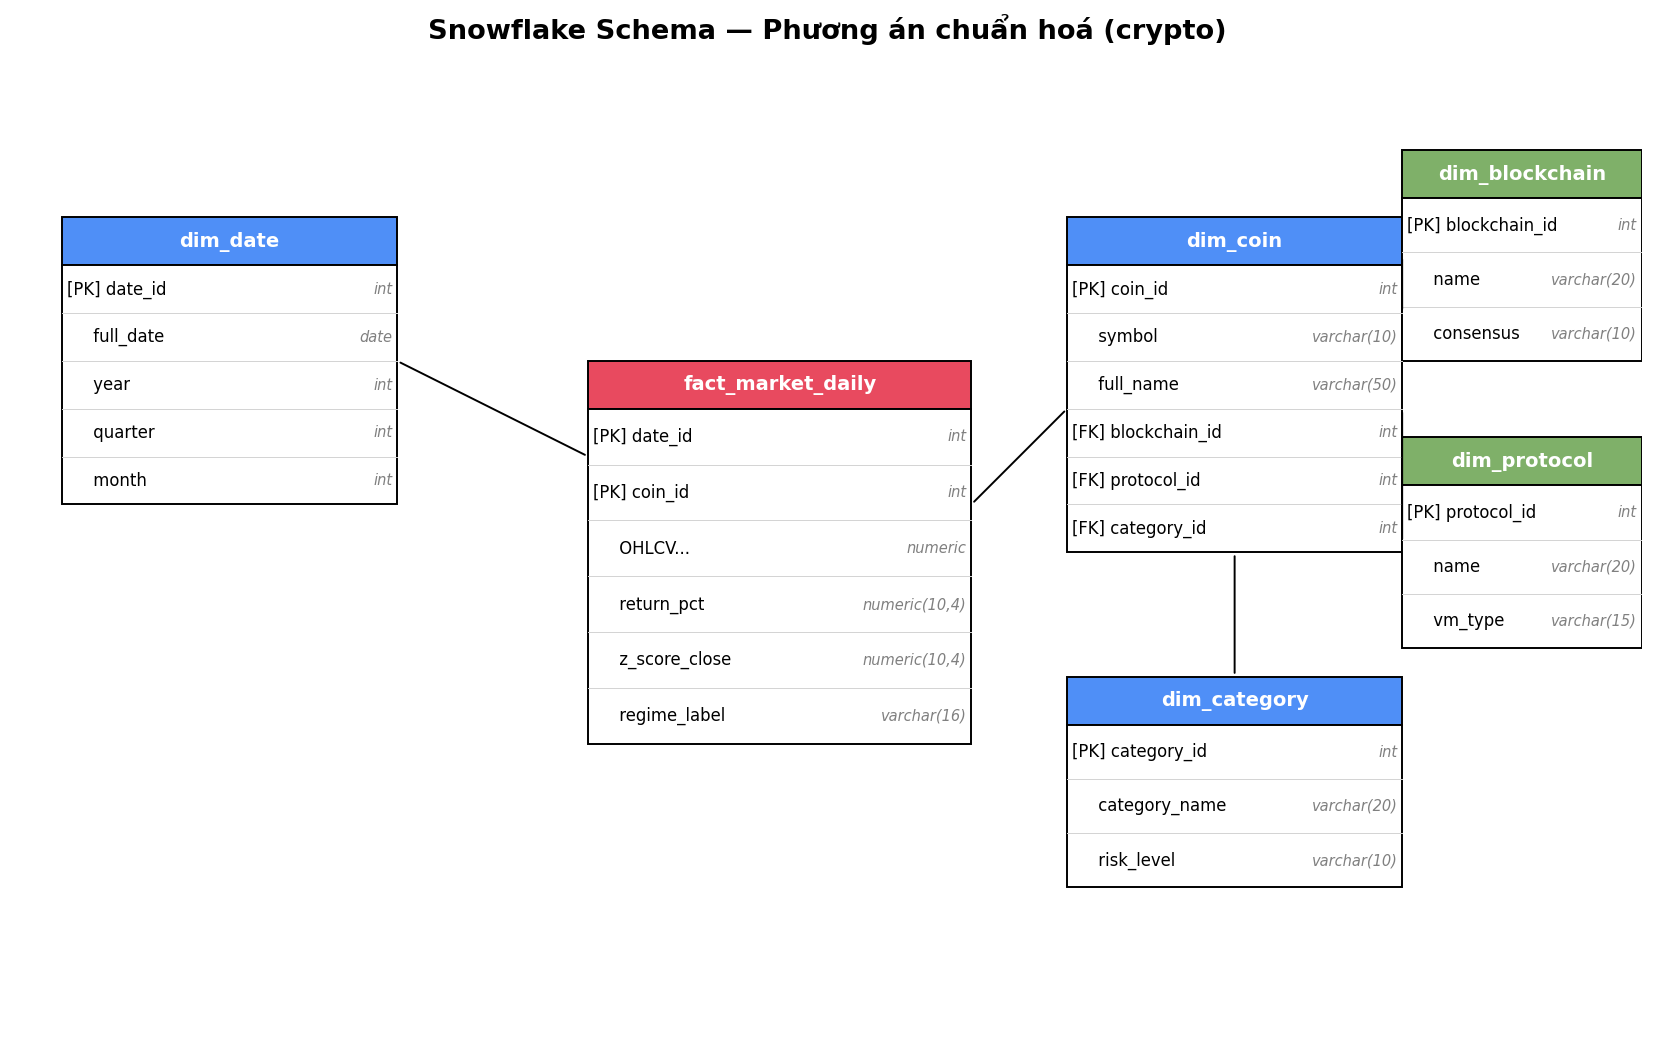
\includegraphics[width=0.9\textwidth]{Images/snowflake-dwh.png}
    \caption{Mô hình kiến trúc Snowflake Schema (Chuẩn hoá)}
    \label{fig:snowflake_schema_design}
\end{figure}

Tuy nhiên với quy mô 10 coin, việc chuẩn hoá thêm sẽ làm tăng số JOIN và phức tạp hoá truy vấn mà không mang lại lợi ích về lưu trữ. Do đó nhóm vẫn chọn Star Schema làm thiết kế chính thức.
